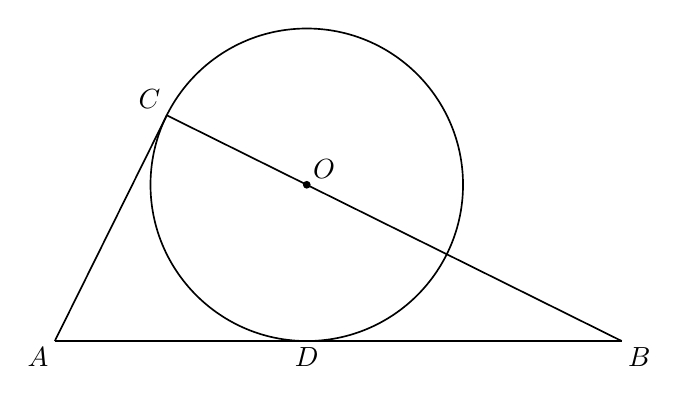
\begin{tikzpicture}[x=1cm,y=1cm,line width=.6pt,font=\normalsize]
\coordinate (O) at (0,1.9845558);
\coordinate (A) at (-3.2,0);
\coordinate (B) at (4,0);
\coordinate (C) at (-1.7777778,2.8665606);
\coordinate (D) at (0,0);
\draw (O) circle[radius=1.9845558cm];
\draw (A)--(C);
\draw (A)--(B);
\draw (C)--(B);
\node[below left=2pt,inner sep=0pt] at (A) {$A$};
\node[above left=2pt,inner sep=0pt] at (C) {$C$};
\node[above right=2pt,inner sep=0pt] at (O) {$O$};
\node[below=2pt,inner sep=0pt] at (D) {$D$};
\node[below right=2pt,inner sep=0pt] at (B) {$B$};

% Explicit named circle-center points, painted after all region fills.
\fill (O) circle[radius=1.4pt];
\end{tikzpicture}
